%%=============================================================================
%% Selectie
%%=============================================================================

\chapter{\IfLanguageName{dutch}{Proof-of-concept}{Proof-of-concept}}%
\label{ch:proof-of-concept}

In dit hoofdstuk wordt de proof-of-concept besproken 
waarbij een beoordeling wordt gevormd van de omgevingen op basis van de performantie metingen.
Allereerst wordt de opzet van de proof-of-concepts voor beide omgevingen besproken.
Hierna worden de performantie metingen uitgevoerd voor beide omgevingen waarna de resultaten worden besproken.
Als laatste worden alle resultaten samengevat om zo te bekijken of Bun een geschikte plaatsvervanger van Node.js kan zijn.

\subsection{Opzet proof-of-concept}
Voor de performantie te meten wordt er per omgeving 2 proof-of-concepts gemaakt. 
Deze metingen zullen worden uitgevoerd op een Mac mini met volgende specificaties:
\begin{itemize}
  \item De Apple M2 chip.
  \item 8GB aan unified memory.
  \item Het macOS Sonoma besturingssysteem
  \item 256GB aan SSD opslag.
  \item Versie 21 van Node.js.
  \item Versie 1.1.3 van Bun.
\end{itemize}
De eerste proof-of-concept zal bestaan uit een script dat het Quick Sort algoritme bevat. 
Deze zal dienen om de computationele verwerking van elke omgeving te beoordelen. Hierbij wordt rekening gehouden met volgende metingen:
\begin{itemize}
    \item De gemiddelde uitvoeringstijd.
    \item Het gemiddelde CPU-gebruik.
    \item Het maximale geheugengebruik.
\end{itemize}
Het Quick Sort algoritme zal een meegegeven array sorteren door een spil element te kiezen binnen de array
waarna de array in 2 arrays wordt opgesplitst. De eerste array zal elementen bevatten die kleiner zijn dan het spil element 
en de andere array zal elementen bevatten die groter zijn. 
De 2 arrays worden vervolgens telkens recursief gesorteerd met dezelfde methode om zo een gesorteerde array te bekomen.
In het codevoorbeeld ~\ref{code:quicksort} kan de code voor het Quick Sort algoritme gevonden worden.
Hierbij is er de mogelijkheid de grootte van de te sorteren array mee te geven via de command-line.

\begin{listing}[H]
    \centering
    \begin{minted}[bgcolor=bg,
        fontfamily=tt,
        linenos=true,
        numberblanklines=true,
        numbersep=5pt,
        gobble=0,
        framesep=2mm,
        tabsize=4,
        obeytabs=false,
        breaklines=true,
        mathescape=false
        samepage=false,
        showspaces=false,
        showtabs =false,
        texcl=false]{js}
const quickSort = (array) => {
  if (array.length <= 1) {
    return array;
  }

  let pivot = array[0];
  let smallArray = [];
  let bigArray = [];

  for (let index = 1; index < array.length; index++) {
    if (array[index] < pivot) {
      smallArray.push(array[index]);
    } else {
      bigArray.push(array[index]);
    }
  }

  return [...quickSort(smallArray), pivot, ...quickSort(bigArray)];
};

const args = process.argv.slice(1); // get length of array
let myArray = Array.from({ length: args[1] }, () =>
  Math.floor(Math.random() * 9)
);
quickSort(myArray);
        \end{minted}
        \caption{\label{code:quicksort}Code voorbeeld quicksort}
\end{listing}

Naast de computationele verwerking te meten, wordt ook de performantie bij I/O-taken gemeten.
Dit wordt gedaan door een proof-of-concept op te stellen die een applicatie back-end voorstelt in de respectievelijke omgeving.
Hierbij kan een gebruiker een lijst van alle onderwerpen ophalen en een recensie creëren over een bepaald onderwerp. 
Binnen de proof-of-concepts zal hierbij getest worden met zowel een Postgres databank als een MySQL databank.
Hierbij wordt rekening gehouden met volgende metingen:
\begin{itemize}
    \item Het gemiddeld aantal verzoeken per seconde die het kan verwerken.
    \item Het gemiddelde CPU-gebruik.
    \item Het maximale geheugengebruik.
    \item De gemiddelde vertraging in de overdracht, ook wel latentie genoemd.
    \item Het aantal gelijktijdige connecties.
    \item Het aantal verzoeken.
    \item De gemiddelde installatietijd.
\end{itemize}
Bij de proof-of-concepts worden enkel de ingebouwde HTTP servers gebruikt om zo beïnvloeding van externe bibliotheken te minimaliseren.
Voor de binnengekomen data naar een database te schrijven wordt een Object Relational Mapper (ORM) gebruikt.
Binnen de applicatie zal voor beide omgevingen gebruikt gemaakt worden van het Sequelize ORM. Deze ondersteunt zowel Postgres als MySQL.
Hierbij worden eerst 3 modellen gemaakt die de volgende tabellen voorstellen in de databank:
\begin{itemize}
  \item Het gebruiker model dat een gebruiker voorstelt.
  \item Het onderwerp model dat een onderwerp voorstelt.
  \item Het recensie model dat de recensie van een bepaalde gebruiker over een bepaald onderwerp voorstelt.
\end{itemize}
De code voor het model van de gebruiker is te vinden in ~\ref{code:User}. Deze bevat 3 kolommen namelijk: de primaire sleutel (id), voornaam en familienaam.
Doormiddel van de sync methode wordt dit model gesynchroniseerd met de database. 
Het model van het onderwerp is gelijkaardig aan de gebruiker zoals te zien is in ~\ref{code:Subject}. Het recensie model heeft bijkomend 
ook nog de 1-op-1 relatie met respectievelijk de gebruiker en het onderwerp.
Om deze relatie tot stand te brengen wordt de belongsTo methode gebruikt in ~\ref{code:Review}. 
Deze zal in de tabel een vreemde sleutel toevoegen naar zowel de gebruiker tabel als de onderwerp tabel. 
\begin{listing}[H]
  \centering
  \begin{minted}[bgcolor=bg,
      fontfamily=tt,
      linenos=true,
      numberblanklines=true,
      numbersep=5pt,
      gobble=0,
      framesep=2mm,
      tabsize=4,
      obeytabs=false,
      breaklines=true,
      mathescape=false
      samepage=false,
      showspaces=false,
      showtabs =false,
      texcl=false]{js}
const { Model, DataTypes  } = require("sequelize");

class Gebruiker extends Model {}

async function GebruikerInit(sequelize) {
  Gebruiker.init(
    {
      id: {
        type: DataTypes.INTEGER,
        autoIncrement: true,
        primaryKey: true,
      },
      voorNaam: {
        type: DataTypes.STRING,
        allowNull: false,
      },
      achterNaam: {
        type: DataTypes.STRING,
      },
    },
    { sequelize, modelName: "Gebruiker" }
  );
  await Gebruiker.sync();
}

module.exports = {
  Gebruiker,
  GebruikerInit,
};
\end{minted}
\caption{\label{code:User}Code van het gebruiker model}
\end{listing}

\begin{listing}[H]
  \centering
  \begin{minted}[bgcolor=bg,
      fontfamily=tt,
      linenos=true,
      numberblanklines=true,
      numbersep=5pt,
      gobble=0,
      framesep=2mm,
      tabsize=4,
      obeytabs=false,
      breaklines=true,
      mathescape=false
      samepage=false,
      showspaces=false,
      showtabs =false,
      texcl=false]{js}
const { Model, DataTypes } = require("sequelize");

class Onderwerp extends Model {}

async function OnderwerpInit(sequelize) {
  Onderwerp.init(
    {
      id: {
        type: DataTypes.INTEGER,
        autoIncrement: true,
        primaryKey: true,
      },
      naam: {
        type: DataTypes.STRING,
        allowNull: false,
      },
    },
    { sequelize, modelName: "Onderwerp" }
  );
  await Onderwerp.sync();
}

module.exports = {
  Onderwerp,
  OnderwerpInit,
};
\end{minted}
\caption{\label{code:Subject}Code van het onderwerp model}
\end{listing}

\begin{listing}[H]
  \centering
  \begin{minted}[bgcolor=bg,
      fontfamily=tt,
      linenos=true,
      numberblanklines=true,
      numbersep=5pt,
      gobble=0,
      framesep=2mm,
      tabsize=4,
      obeytabs=false,
      breaklines=true,
      mathescape=false
      samepage=false,
      showspaces=false,
      showtabs =false,
      texcl=false]{js}
const { Model, DataTypes } = require("sequelize");
const { Gebruiker } = require("./gebruiker.js");
const { Onderwerp } = require("./onderwerp.js");
class Recensie extends Model {}

module.exports = async (sequelize) => {
  Recensie.init(
    {
      id: {
        type: DataTypes.INTEGER,
        autoIncrement: true,
        primaryKey: true,
      },
      bericht: {
        type: DataTypes.STRING,
        allowNull: false,
      },
    },
    { sequelize, modelName: "Recensie" }
  );
  Recensie.belongsTo(Gebruiker, { onDelete: "CASCADE" });
  Recensie.belongsTo(Onderwerp, { onDelete: "CASCADE" });
  await Recensie.sync();
};
\end{minted}
\caption{\label{code:Review}Code van het recensie model}
\end{listing}

In de code ~\ref{code:Instantie} wordt een connectie aangemaakt met de databank door het gebruik van Sequelize. 
De benodigde configuratie wordt met behulp van de config package opgehaald. Zo is de 
gebruikersnaam, databasenaam en de technologie van de database te vinden in de configuratie bestanden.
Voor zowel te kunnen werken met MySQL als Postgres wordt gebruikgemaakt van de packages: mysql2 en pg.
Het wachtwoord zal dankzij de config package opgehaald worden uit het environment om zo de veiligheid te waarborgen.
Deze configuratie wordt dan gebruikt om de connectie aan te maken en de tabellen te initializeren.
Nadien worden ook de gebruiker en onderwerp tabel opgevuld met voorbeeld data zoals te zien is in ~\ref{code:Seed}.

\begin{listing}[H]
  \centering
  \begin{minted}[bgcolor=bg,
      fontfamily=tt,
      linenos=true,
      numberblanklines=true,
      numbersep=5pt,
      gobble=0,
      framesep=2mm,
      tabsize=4,
      obeytabs=false,
      breaklines=true,
      mathescape=false
      samepage=false,
      showspaces=false,
      showtabs =false,
      texcl=false]{js}
const { Sequelize } = require("sequelize");
const configuration = require("config");
const RecensieMigratie = require("./recensie");
const seed = require("./seeder");
const { GebruikerInit } = require("./gebruiker");
const { OnderwerpInit } = require("./onderwerp");
//config
const username = configuration.get("development.username");
const database = configuration.get("development.database");
const dialect = configuration.get("development.dialect");
const password = configuration.get("password");

// Instantie aanmaken
let sequelize;
async function initializeSequelize() {
  sequelize = new Sequelize(database, username, password, {
    host: "mysql",
    dialect: dialect,
  });
  try {
    await sequelize.authenticate();
    console.log("Connection has been established successfully.");
  } catch (error) {
    console.error("Unable to connect to the database:", error);
  }
  await GebruikerInit(sequelize);
  await OnderwerpInit(sequelize);
  await RecensieMigratie(sequelize);
  await seed(sequelize);
  return sequelize;
}

function getSequelize() {
  if (!sequelize) {
    throw new Error("initialize sequelize");
  }
  return sequelize;
}
module.exports = {
  initializeSequelize,
  getSequelize,
};
\end{minted}
\caption{\label{code:Instantie}Code bij aanmaken instantie sequelize}
\end{listing}

\begin{listing}[H]
  \centering
  \begin{minted}[bgcolor=bg,
      fontfamily=tt,
      linenos=true,
      numberblanklines=true,
      numbersep=5pt,
      gobble=0,
      framesep=2mm,
      tabsize=4,
      obeytabs=false,
      breaklines=true,
      mathescape=false
      samepage=false,
      showspaces=false,
      showtabs =false,
      texcl=false]{js}
async function seed(sequelize) {
  // Originele staat
  await sequelize.models.Gebruiker.destroy({ truncate: { cascade: true } });
  await sequelize.models.Onderwerp.destroy({ truncate: { cascade: true } });
  await sequelize.models.Gebruiker.create({
    id: 1,
    voorNaam: "Quinten",
    achterNaam: "De Wolf",
  });
  await sequelize.models.Onderwerp.create({
    id: 1,
    naam: "Cars",
  });
  await sequelize.models.Onderwerp.create({
    id: 2,
    naam: "Planes",
  });
  await sequelize.models.Onderwerp.create({
    id: 3,
    naam: "Racing",
  });
}
module.exports = seed;
\end{minted}
\caption{\label{code:Seed}Code bij het opvullen van de tabellen}
\end{listing}

Als laatste wordt de server aangemaakt om een POST methode op het recensie endpoint en een GET methode op het onderwerpen endpoint aan te nemen.
In ~\ref{code:NodeServer} wordt de code om dit te bereiken in Node.js getoond. Hierbij komt data in de vorm van JSON binnen voor de POST methode.
Deze bevat de recensie in combinatie met het id van het onderwerp en de gebruiker.
Deze zal dan gebruikt worden om een nieuwe rij aan te maken in de recensie tabel.
Daarnaast is er ook een GET endpoint die de lijst van alle onderwerpen zal ophalen en teruggeven.
In ~\ref{code:BunServer} kan dezelfde functionele code worden gevonden voor Bun.

\begin{listing}[H]
  \centering
  \begin{minted}[bgcolor=bg,
      fontfamily=tt,
      linenos=true,
      numberblanklines=true,
      numbersep=5pt,
      gobble=0,
      framesep=2mm,
      tabsize=4,
      obeytabs=false,
      breaklines=true,
      mathescape=false
      samepage=false,
      showspaces=false,
      showtabs =false,
      texcl=false]{js}
const http = require("node:http");
const { initializeSequelize } = require("./sequelize.js");
async function main() {
  const sequelizeInstance = await initializeSequelize();
  http
    .createServer(async (req, res) => {
      if (req.method === "POST" && req.url === "/recensie") {
        let body = "";
        req.on("data", (data) => {
          body += data.toString(); 
        });
        req.on("end", async () => {
          try {
            const data = JSON.parse(body);
            await sequelizeInstance.models.Recensie.create(data);
            res.writeHead(201, { "Content-Type": "application/json" });
            res.end();
          } catch (error) {
            console.error("Error:", error);
            res.writeHead(400, { "Content-Type": "application/json" });
            res.end(JSON.stringify({ message: "Invalid data" }));
          }
        });
      } else if (req.method === "GET" && req.url === "/onderwerpen") {
        try {
          const data = await sequelizeInstance.models.Onderwerp.findAll();
          res.writeHead(200, { "Content-Type": "application/json" });
          res.end(JSON.stringify(data));
        } catch {
          res.writeHead(500, { "Content-Type": "tet/plain" });
          res.end('Internal Server error')
        }
      }
    })
    .listen(3000);
}
main();
\end{minted}
\caption{\label{code:NodeServer}Code om de verzoeken te ontvangen binnen Node.js}
\end{listing}
\begin{listing}[H]
  \centering
  \begin{minted}[bgcolor=bg,
      fontfamily=tt,
      linenos=true,
      numberblanklines=true,
      numbersep=5pt,
      gobble=0,
      framesep=2mm,
      tabsize=4,
      obeytabs=false,
      breaklines=true,
      mathescape=false
      samepage=false,
      showspaces=false,
      showtabs =false,
      texcl=false]{js}
const { initializeSequelize } = require("./sequelize.js");
const sequelizeInstance = await initializeSequelize();
Bun.serve({
    port:3000,
    async fetch(request) {
        try {
            const url = new URL(request.url);
            if (request.method === "POST" && url.pathname === "/recensie") {
                const data = await request.json();
                await sequelizeInstance.models.Recensie.create(data);
                return new Response('',{headers: { "Content-Type": "application/json"}, status: 201});
            } else if (request.method === "GET" && url.pathname === "/onderwerpen") {
                const data = await sequelizeInstance.models.Onderwerp.findAll();
                return Response.json(data);
            }
        } catch (error) {
            console.error("Error:", error);
            return new Response(JSON.stringify({ message: 'Invalid data'}), 
            {headers: { "Content-Type": "application/json"}, status: 400})
        }
    }
})
\end{minted}
\caption{\label{code:BunServer}Code om de verzoeken te ontvangen binnen server}
\end{listing}
\subsection{Uitvoering metingen}
Voor de metingen wordt gebruikgemaakt van 2 hulpprogramma's: Hyperfine en Bombardier.
In \ref{code:HyperfineScript} wordt Hyperfine gebruikt om de gemiddelde uitvoeringstijd over verschillende iteraties van het script te berekenen.
Ook zal Hyperfine gebruikt worden om de gemiddelde installatietijd van de respectievelijke package managers te vergelijken zoals 
te zien is in \ref{code:HyperfineInstall}. Specifiek wordt de installatietijd bekeken wanneer het cache geheugen data bevat.
Bij de metingen wordt telkens versie 1.18 van Hyperfine gebruikt.
\begin{listing}[H]
  \centering
  \begin{minted}[bgcolor=bg,
      fontfamily=tt,
      linenos=true,
      numberblanklines=true,
      numbersep=5pt,  
      gobble=0,
      framesep=2mm,
      tabsize=4,
      obeytabs=false,
      breaklines=true,
      mathescape=false
      samepage=false,
      showspaces=false,
      showtabs =false,
      texcl=false]{shell-session}
> hyperfine 'node index.js 1000' 'bun index.js 1000'
      \end{minted}
      \caption{\label{code:HyperfineScript}Gebruik Hyperfine commando bij het script}
\end{listing}

\begin{listing}[H]
  \centering
  \begin{minted}[bgcolor=bg,
      fontfamily=tt,
      linenos=true,
      numberblanklines=true,
      numbersep=5pt,  
      gobble=0,
      framesep=2mm,
      tabsize=4,
      obeytabs=false,
      breaklines=true,
      mathescape=false
      samepage=false,
      showspaces=false,
      showtabs =false,
      texcl=false]{shell-session}
> hyperfine --prepare 'rm -rf node_modules' --warmup 1 --runs 100 'npm install' 'bun install'
      \end{minted}
      \caption{\label{code:HyperfineInstall}Gebruik Hyperfine commando bij het script}
\end{listing}
Daarnaast wordt voor de HTTP server gebruikgemaakt van Bombardier. 
Hierbij kan ingesteld worden hoeveel gelijktijdige connecties er zijn en hoeveel verzoeken per test worden verstuurd.
In de metingen zal getest worden door 500000 verzoeken te sturen met 10, 100 en 1000 gelijktijdige connecties.
De commando's hiervoor zijn terug te vinden in \ref{code:Bombardier10}, \ref{code:Bombardier100} en \ref{code:Bombardier1000}.
Hierbij wordt telkens een POST verzoek gestuurd, in \ref{code:Bombardier10GET} wordt een voorbeeld getoond om GET verzoeken te sturen.
Bij de metingen wordt hiervoor gebruikgemaakt van versie 1.2.6 van Bombardier.
\begin{listing}[H]
  \centering
  \begin{minted}[bgcolor=bg,
      fontfamily=tt,
      linenos=true,
      numberblanklines=true,
      numbersep=5pt,  
      gobble=0,
      framesep=2mm,
      tabsize=4,
      obeytabs=false,
      breaklines=true,
      mathescape=false
      samepage=false,
      showspaces=false,
      showtabs =false,
      texcl=false]{shell-session}
> bombardier -c 10 -n 500000 -m POST -b '{"bericht": "test","GebruikerId": 1,"OnderwerpId": 1}' -l http://localhost:3000/recensie
      \end{minted}
      \caption{\label{code:Bombardier10}Gebruik Bombardier commando met 500000 verzoeken en 10 gelijktijdige connecties voor een POST verzoek}
\end{listing}
\begin{listing}[H]
  \centering
  \begin{minted}[bgcolor=bg,
      fontfamily=tt,
      linenos=true,
      numberblanklines=true,
      numbersep=5pt,  
      gobble=0,
      framesep=2mm,
      tabsize=4,
      obeytabs=false,
      breaklines=true,
      mathescape=false
      samepage=false,
      showspaces=false,
      showtabs =false,
      texcl=false]{shell-session}
> bombardier -c 100 -n 500000 -m POST -b '{"bericht": "test","GebruikerId": 1,"OnderwerpId": 1}' -l http://localhost:3000/recensie
      \end{minted}
      \caption{\label{code:Bombardier100}Gebruik Bombardier commando met 500000 verzoeken en 100 gelijktijdige connecties voor een POST verzoek}
\end{listing}
\begin{listing}[H]
  \centering
  \begin{minted}[bgcolor=bg,
      fontfamily=tt,
      linenos=true,
      numberblanklines=true,
      numbersep=5pt,  
      gobble=0,
      framesep=2mm,
      tabsize=4,
      obeytabs=false,
      breaklines=true,
      mathescape=false
      samepage=false,
      showspaces=false,
      showtabs =false,
      texcl=false]{shell-session}
> bombardier -c 1000 -n 500000 -m POST -b '{"bericht": "test","GebruikerId": 1,"OnderwerpId": 1}' -l http://localhost:3000/recensie
      \end{minted}
      \caption{\label{code:Bombardier1000}Gebruik Bombardier commando met 500000 verzoeken en 1000 gelijktijdige connecties voor een POST verzoek}
\end{listing}
\begin{listing}[H]
  \centering
  \begin{minted}[bgcolor=bg,
      fontfamily=tt,
      linenos=true,
      numberblanklines=true,
      numbersep=5pt,  
      gobble=0,
      framesep=2mm,
      tabsize=4,
      obeytabs=false,
      breaklines=true,
      mathescape=false
      samepage=false,
      showspaces=false,
      showtabs =false,
      texcl=false]{shell-session}
> bombardier -c 10 -n 500000 -l http://localhost:3000/onderwerpen
      \end{minted}
      \caption{\label{code:Bombardier10GET}Gebruik Bombardier commando met 500000 verzoeken en 10 gelijktijdige connecties voor een GET verzoek}
\end{listing}
Bij de uitvoering wordt gewerkt met een vorm van containervirtualisatie genaamd Docker.
Hierbij zit elke aplicatie in zijn eigen container waarbij aan de hand van een Dockerfile deze telkens wordt opgezet.
In \ref{code:dockerscript} is de Dockerfile voor het Quick Sort algoritme te zien. 
Hierbij wordt vertrokken van een omgeving die Node.js al bevat waar nadien Hyperfine en Bun worden geïnstalleerd.
Hierna wordt dan met behulp van Hyperfine de uitvoeringstijd van Bun en Node.js berekend.
Dit bestand moet eerst gebouwd worden met het docker build commando waarvan een voorbeeld te vinden is in \ref{code:dockerbuild}.
Daarna moet de image worden uitgevoerd met het docker run commando zoals het voorbeeld in \ref{code:dockerrun}.
Voor de HTTP server is er nog een bijkomend
Docker Compose bestand \ref{code:dockerscript} waar aan de hand van het commando in \ref{code:dockercompose}
zowel de databank als de server kan worden opgestart. Een voorbeeld hiervan voor een mysql database is te zien in \ref{code:dockercompose}.
Hiernaast wordt dan ook een Dockerfile gebruikt om de server te starten. De Dockerfile voor de Node.js en Bun server is te vinden in
respectievelijk \ref{code:dockernode} en \ref{code:dockerbun}. 
Om het gemiddelde CPU-gebruik en het maximale geheugengebruik te bepalen wordt het bombardier commando samen met het docker stats commando uitgevoerd in een zsh script.
Hierbij wordt voordat het bombardier commando wordt uitgevoerd de monitoring gestart van het geheugen en het cpu-gebruik. Nadien wordt het gemiddelde cpu-gebruik en het maximale geheugen gebruik bepaald.
Een voorbeeld van dit script  is te vinden in \ref{code:zshscript}. 
In dit voorbeeld wordt zowel de bombardier om de POST methode als de GET methode weergegeven. Afhankelijk van wat gemeten wordt, moet tussen 1 van deze 2 methoden gekozen worden.
Het aantal connecties kan als argument meegegeven worden bij de uitvoering van het script.
Daarnaast wordt bij de server ook de installatietijd van de package managers gemeten met de Dockerfile \ref{code:dockerinstall}.
Hiervoor wordt ook Hyperfine gebruikt waarbij de cache al wordt opgevuld door de warmup in het commando.
\begin{listing}[H]
  \centering
  \begin{minted}[bgcolor=bg,
      fontfamily=tt,
      linenos=true,
      numberblanklines=true,
      numbersep=5pt,  
      gobble=0,
      framesep=2mm,
      tabsize=4,
      obeytabs=false,
      breaklines=true,
      mathescape=false
      samepage=false,
      showspaces=false,
      showtabs =false,
      texcl=false]{bash}
# Base image met Node.js geïnstalleerd
FROM node:21

# Installeer Hyperfine met apt
RUN apt-get update && \
    apt-get install -y curl && \
    apt-get install -y hyperfine

RUN curl -fsSL https://bun.sh/install | bash && \
  ln -s $HOME/.bun/bin/bun /usr/local/bin/bun
# Zet de werk map in de container
WORKDIR /app

# Kopieer de applicatie code naar de container
COPY . .
RUN ~/.bun/bin/bun install
# Commando dat wordt uitgevoerd wanneer container start
CMD ["hyperfine","node index.js 1000", "bun index.js 1000"]
      \end{minted}
      \caption{\label{code:dockerscript}Dockerfile voor het Quick Sort algoritme}
\end{listing}
\begin{listing}[H]
  \centering
  \begin{minted}[bgcolor=bg,
      fontfamily=tt,
      linenos=true,
      numberblanklines=true,
      numbersep=5pt,  
      gobble=0,
      framesep=2mm,
      tabsize=4,
      obeytabs=false,
      breaklines=true,
      mathescape=false
      samepage=false,
      showspaces=false,
      showtabs =false,
      texcl=false]{shell-session}
> docker build -f "Dockerfile" -t testimage .
      \end{minted}
      \caption{\label{code:dockerbuild}Voorbeeld bouwen van een docker image met naam testimage}
\end{listing}
\begin{listing}[H]
  \centering
  \begin{minted}[bgcolor=bg,
      fontfamily=tt,
      linenos=true,
      numberblanklines=true,
      numbersep=5pt,  
      gobble=0,
      framesep=2mm,
      tabsize=4,
      obeytabs=false,
      breaklines=true,
      mathescape=false
      samepage=false,
      showspaces=false,
      showtabs =false,
      texcl=false]{shell-session}
> docker run -it testimage .
      \end{minted}
      \caption{\label{code:dockerrun}Voorbeeld uitvoeren van een docker image met naam testimage}
\end{listing}

\begin{listing}[H]
  \centering
  \begin{minted}[bgcolor=bg,
      fontfamily=tt,
      linenos=true,
      numberblanklines=true,
      numbersep=5pt,  
      gobble=0,
      framesep=2mm,
      tabsize=4,
      obeytabs=false,
      breaklines=true,
      mathescape=false
      samepage=false,
      showspaces=false,
      showtabs =false,
      texcl=false]{shell-session}
> docker-compose up --build
      \end{minted}
      \caption{\label{code:dockercompose}Uitvoeren van een docker compose}
\end{listing}
\begin{listing}[H]
  \centering
  \begin{minted}[bgcolor=bg,
      fontfamily=tt,
      linenos=true,
      numberblanklines=true,
      numbersep=5pt,  
      gobble=0,
      framesep=2mm,
      tabsize=4,
      obeytabs=false,
      breaklines=true,
      mathescape=false
      samepage=false,
      showspaces=false,
      showtabs =false,
      texcl=false]{yaml}
version: '3'

services:
mysql:
  image: mysql:latest
  environment:
    MYSQL_ROOT_PASSWORD: Test12345
    MYSQL_DATABASE: review
  ports:
    - "3306:3306"
  healthcheck:
    test: ["CMD", "mysqladmin", "ping", "-h", "localhost"]
    interval: 5s
    timeout: 3s
    retries: 5

server:
  build: .
  depends_on:
    mysql:
      condition: service_healthy
  ports:
    - "3000:3000"
  environment:
    MYSQL_HOST: mysql
    MYSQL_PORT: 3306
    MYSQL_USER: root
    MYSQL_PASSWORD: Test12345
    MYSQL_DATABASE: review
      \end{minted}
      \caption{\label{code:dockercompose}Docker Compose bestand voor het opstarten van de mysql database en server}
\end{listing}

\begin{listing}[H]
  \centering
  \begin{minted}[bgcolor=bg,
      fontfamily=tt,
      linenos=true,
      numberblanklines=true,
      numbersep=5pt,  
      gobble=0,
      framesep=2mm,
      tabsize=4,
      obeytabs=false,
      breaklines=true,
      mathescape=false
      samepage=false,
      showspaces=false,
      showtabs =false,
      texcl=false]{bash}
# Base image met Node.js geïnstalleerd
FROM node:21

# Zet de werk map in de container
WORKDIR /app

# Kopieer de package.json and package-lock.json bestanden naar de container
COPY package*.json ./

# Installeer dependencies
RUN npm install

# Kopieer de rest van de applicatie code naar de container
COPY . .

# Zet de poort open
EXPOSE 3000

# Commando dat wordt uitgevoerd wanneer container start
CMD ["npm", "run", "dev"]
      \end{minted}
      \caption{\label{code:dockernode}Dockerfile voor de node server}
\end{listing}


\begin{listing}[H]
  \centering
  \begin{minted}[bgcolor=bg,
      fontfamily=tt,
      linenos=true,
      numberblanklines=true,
      numbersep=5pt,  
      gobble=0,
      framesep=2mm,
      tabsize=4,
      obeytabs=false,
      breaklines=true,
      mathescape=false
      samepage=false,
      showspaces=false,
      showtabs =false,
      texcl=false]{bash}
# Base image met bun geïnstalleerd
FROM oven/bun:1.1.3 as base

# Zet de werk map in de container
WORKDIR /usr/src/app

# Kopieer de package.json and package-lock.json bestanden naar de container
COPY package.json bun.lockb ./
# Installeer dependencies
RUN bun install

# Kopieer de rest van de applicatie code naar de container
COPY . .

# Zet de poort open
EXPOSE 3000

# Commando dat wordt uitgevoerd wanneer container start
CMD ["bun", "run", "index.js"]
      \end{minted}
      \caption{\label{code:dockerbun}Dockerfile voor de bun server}
\end{listing}

\begin{listing}[H]
  \centering
  \begin{minted}[bgcolor=bg,
      fontfamily=tt,
      linenos=true,
      numberblanklines=true,
      numbersep=5pt,  
      gobble=0,
      framesep=2mm,
      tabsize=4,
      obeytabs=false,
      breaklines=true,
      mathescape=false
      samepage=false,
      showspaces=false,
      showtabs =false,
      texcl=false]{bash}
#!/bin/zsh

# Start de monitoring
docker stats <container_naam> --format "table {{.Container}}\t{{.CPUPerc}}\t{{.MemUsage}}" > container_stats.txt &

# Start bombardier POST
bombardier -c "$1" -n 500000 -m POST -b '{"bericht": "test","GebruikerId": 1,"OnderwerpId": 1}' -l http://localhost:3000/recensie
# Of
# Start bombardier GET
bombardier -c "$1" -n 500000 -l http://localhost:3000/onderwerpen

# Stop de docker stats

target_command="/Applications/Docker.app/Contents/Resources
/bin/com.docker.cli stats"
docker_cli_pid=$(ps aux | grep "$target_command" | grep -v grep | awk '{print $2}')

if [[ -n $docker_cli_pid ]]; then
    echo "Killing Docker CLI process with PID: $docker_cli_pid"
    kill -9 $docker_cli_pid
else
    echo "Docker CLI process not found."
fi


# Bereken gemiddeld CPU-gebruik en hoogste memory
while IFS= read -r line; do
    if [[ $line =~ ([0-9]+\.[0-9]+)%(.*[0-9]+\.[0-9]+)MiB ]]; then
        cpu_percent="${match[1]}"
        mem_usage="${match[2]}"
        cpu_percent_sum=$((cpu_percent_sum + cpu_percent))
        if (( mem_usage > highest_mem_usage )); then
            highest_mem_usage="$mem_usage"
        fi
        ((total_lines++))
    fi
done < container_stats.txt

average_cpu_percent=$((cpu_percent_sum / total_lines))

# Toon resultaten
echo "Gemiddelde CPU-gebruik: $average_cpu_percent%"
echo "Maximaal geheugen gebruik: $highest_mem_usage"

      \end{minted}
      \caption{\label{code:zshscript}Dockerfile voor het Quick Sort algoritme}
\end{listing}

\begin{listing}[H]
  \centering
  \begin{minted}[bgcolor=bg,
      fontfamily=tt,
      linenos=true,
      numberblanklines=true,
      numbersep=5pt,  
      gobble=0,
      framesep=2mm,
      tabsize=4,
      obeytabs=false,
      breaklines=true,
      mathescape=false
      samepage=false,
      showspaces=false,
      showtabs =false,
      texcl=false]{bash}
# Base image met Node.js geïnstalleerd
FROM node:21

# Installeer Hyperfine met apt
RUN apt-get update && \
    apt-get install -y curl && \
    apt-get install -y hyperfine

RUN curl -fsSL https://bun.sh/install | bash && \
  ln -s $HOME/.bun/bin/bun /usr/local/bin/bun
# Zet de werk map in de container
WORKDIR /app

# Kopieer de applicatiebestanden naar de container
COPY . .
RUN ~/.bun/bin/bun install
# Commando dat wordt uitgevoerd wanneer container start
CMD ["hyperfine","--prepare", "rm -rf node_modules", "--warmup","1","--runs","100","bun install","npm install"]
      \end{minted}
      \caption{\label{code:dockerinstall}Dockerfile voor de installatietijd te meten bij de server}
\end{listing}

\subsection{Resultaten proof-of-concept}
In deze sectie zullen de resultaten van de performantie testen besproken worden.
Hierbij worden eerst de resultaten voor de uitvoeringstijd, cpu-gebruik en geheugengebruik bij het Quick Sort algoritme bekeken.
Daarna worden de resultaten van de server besproken op vlak van uitvoeringstijd, cpu-gebruik, geheugengebruik, latentie en de installatietijd.

\subsubsection{Resultaten  Quick Sort algoritme}
De resultaten voor de gemiddelde uitvoeringstijd bij het Quick Sort algoritme werden bekomen doormiddel van Hyperfine.
Hierbij werd gekeken naar de uitvoeringstijd voor het sorteren van een array bestaande uit 1000 elementen met volgend commando \ref{code:HyperfineScript}.
In figuur \ref{fig:uitvoeringstijdscript} wordt de gemiddelde uitvoeringstijd per omgeving visueel voorgesteld. 
Daarbij is op te merken dat de gemiddelde uitvoeringstijd van Bun gemiddeld 2.21 keer sneller is dan bij Node.js.
\begin{figure}[H]
  \centering
  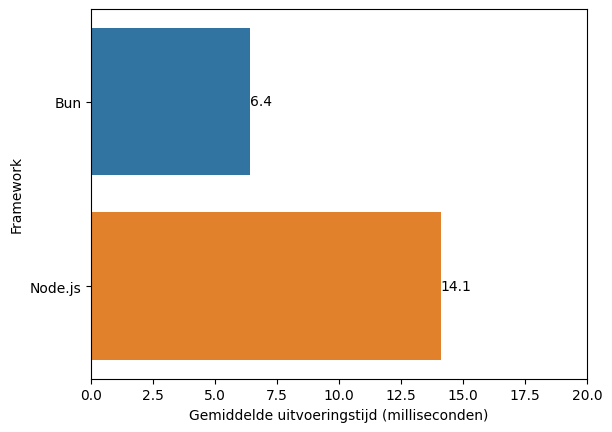
\includegraphics{graphics/scriptuitvoeringstijd.png}
  \caption{\label{fig:uitvoeringstijdscript}Gemiddelde uitvoeringstijd van het Quick Sort algoritme voor Bun en Node.js}
\end{figure}

\subsection{Resultaten Recensie applicatie}
De resultaten voor de gemiddelde installatietijd werden bekomen doormiddel van Hyperfine.
Hierbij werd eerst een warmup uitvoering gedaan om de cache al op te vullen.
In figuur \ref{fig:installatietijdapp} zijn de resultaten visueel voorgesteld per omgeving.
Hierbij is op te merken dat Bun met een gemiddelde installatietijd van 24,9 milliseconden 24,5 keer sneller 
is dan Node.js met een gemiddelde installatietijd van 610,1 milleseconden.
\begin{figure}[H]
  \centering
  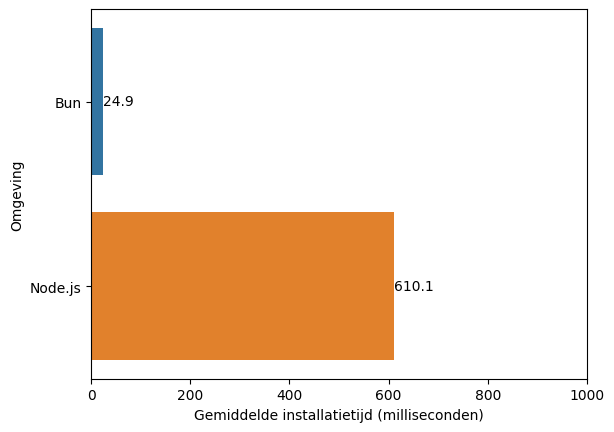
\includegraphics{graphics/install.png}
  \caption{\label{fig:installatietijdapp}Gemiddelde installatietijd van de packages in Bun en Node.js}
\end{figure}

Voor de andere resultaten werd gebruikgemaakt van Bombardier waarbij telkens met 10, 100 en 1000 connecties 
500000 verzoeken werden gestuurd naar de server.
In tabel \ref{tab:getbombardier} kunnen de resultaten gezien worden van de metingen waarbij de onderwerpen werden opgehaald aan de hand van een GET verzoek.
Er wordt gestreefd naar een zo hoog mogelijk aantal verzoeken per seconde met een zo laag mogelijke latentie, geheugengebruik en cpu-gebruik.
Zoals te zien scoort Bun op het vlak van aantal verzoeken per seconde en latentie beter dan Node.js ongeacht van het aantal connecties. 
Echter heeft Bun bij het aantal verzoeken per seconde wel telkens een grotere standaardafwijking en er dus meer uitschieters aanwezig zijn.
Langs de andere kant verbruikt Bun telkens meer resources. Zo heeft Bun bij elke connectie een hoger CPU-gebruik en zijn de pieken van het geheugen consistent hoger dan bij Node.js.
In figuren \ref{fig:getaantalverzoekenmysql}, \ref{fig:getaantallatentienmysql}, \ref{fig:getgeheugennmysq} en \ref{fig:getcpymysql} kunnen de visuele voorstellingen 
voor respectievelijk het aantal verzoeken per seconde, het aantal latentie, het maximale geheugengebruik en het gemiddeld CPU-gebruik worden gevonden.
\begin{table}[]
  \begin{tabular}{|c|cccccc|}
  \hline
  \multicolumn{1}{|l|}{}                                                                     & \multicolumn{1}{l}{} & Bun     & \multicolumn{1}{l|}{}     & \multicolumn{1}{l}{} & \multicolumn{1}{l}{Node.js} & \multicolumn{1}{l|}{} \\ \hline
  Aantal connecties                                                                          & 10                   & 100     & \multicolumn{1}{c|}{1000} & 10                   & 100                         & 1000                  \\ \hline
  \begin{tabular}[c]{@{}c@{}}Gemiddeld aantal \\ verzoeken per seconde\end{tabular}          & 8531.89              & 7441.10 & 7905.77                   & 7643.59              & 7138.43                     & 6443.86               \\ \cline{1-1}
  \begin{tabular}[c]{@{}c@{}}Standaardafwijking aantal \\ verzoeken per seconde\end{tabular} & 2712.38              & 2308.74 & 2475.46                   & 2387.87              & 1682.46                     & 1798.40               \\ \cline{1-1}
  \begin{tabular}[c]{@{}c@{}}Latentie \\ (milliseconden)\end{tabular}                        & 1.17                 & 13.05   & 144.70                    & 1.31                 & 14.01                       & 155.10                \\ \cline{1-1}
  \begin{tabular}[c]{@{}c@{}}Standaardafwijking\\ latentie\\ (milliseconden)\end{tabular}    & 0.66809              & 2.62    & 22.61                     & 0.89                 & 2.57                        & 42.51                 \\ \cline{1-1}
  \begin{tabular}[c]{@{}c@{}}Maximale \\ geheugengebruik \\ (MB)\end{tabular}                & 152.3                & 223.2   & 242.6                     & 80.75                & 88.25                       & 130.3                 \\ \cline{1-1}
  \begin{tabular}[c]{@{}c@{}}Gemiddeld\\ CPU-gebruik\\ (\%)\end{tabular}                     & 110.90               & 137.26  & 137.52                    & 98.2                 & 102.33                      & 120.39                \\ \hline
  \end{tabular}
  \caption{\label{tab:getbombardier}Resultaten metingen waarbij onderwerpen worden opgehaald met een GET request.}
  \end{table}

  \begin{figure}[H]
    \centering
    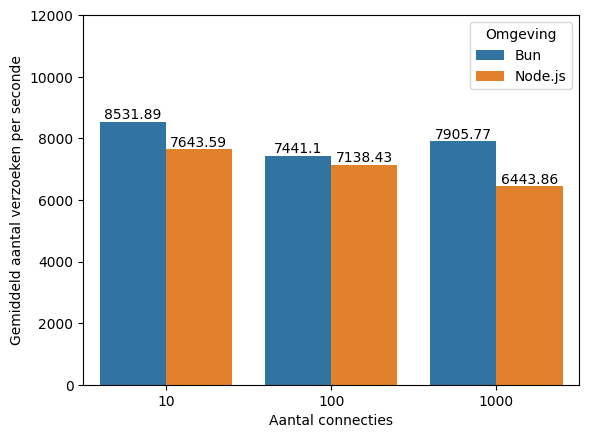
\includegraphics{graphics/GetMySqlVerzoeken.png}
    \caption{\label{fig:getaantalverzoekenmysql}Visuele voorstelling gemiddeld aantal verzoeken per seconde bij het ophalen van de onderwerpen.}
  \end{figure}
  \begin{figure}[H]
    \centering
    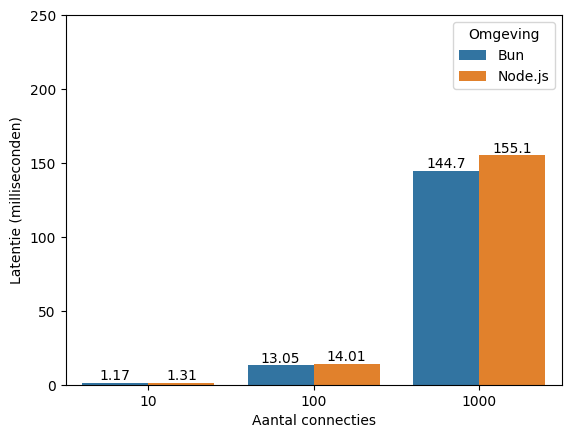
\includegraphics{graphics/GetMySqlLatentie.png}
    \caption{\label{fig:getaantallatentienmysql}Visuele voorstelling gemiddelde latentie bij het ophalen van de onderwerpen.}
  \end{figure}
  \begin{figure}[H]
    \centering
    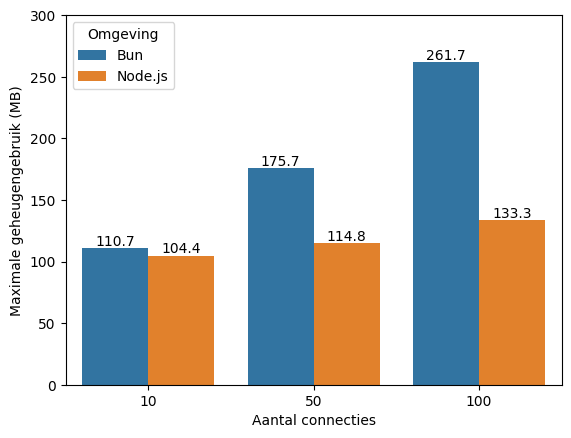
\includegraphics{graphics/GetMySqlRAM.png}
    \caption{\label{fig:getgeheugennmysql}Visuele voorstelling maximale geheugen gebruik bij het ophalen van de onderwerpen.}
  \end{figure}
  \begin{figure}[H]
    \centering
    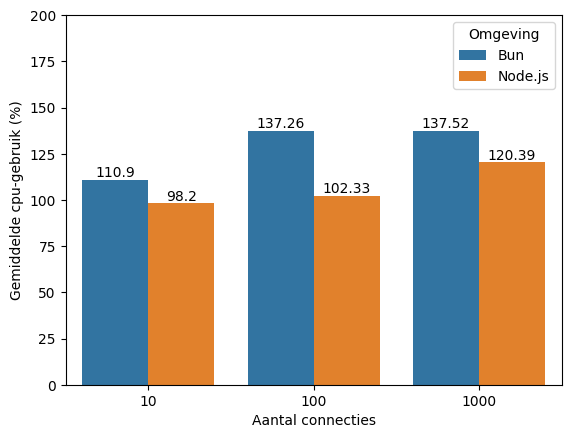
\includegraphics{graphics/GetMySqlCpu.png}
    \caption{\label{fig:getcpymysql}Visuele voorstelling gemiddeld CPU-gebruik bij het ophalen van de onderwerpen.}
  \end{figure}

In In tabel \ref{tab:postbombardier} kunnen de resultaten gezien worden van de metingen waarbij 
een gebruiker een recensie schrijft over een bepaald onderwerp door gebruik van een POST verzoek.
Hierbij is op te merken dat Bun op alle vlakken slechter scoort dan Node.js. Zo heeft bijvoorbeeld bij 10 connecties Bun
een lager gemiddeld aantal verzoeken (M = 3298.09; SD = 814.04) dan Node.js (M = 3794.32; SD = 855.81) en een hogere latentie (M = 3.03; SD = 1.42) 
ondanks het feit dat het gemiddeld CPU-gebruik en maximale geheugengebruik hoger ligt.
In figuren \ref{fig:postaantalverzoekenmysql}, \ref{fig:postaantallatentienmysql}, \ref{fig:postgeheugennmysq} en \ref{fig:postcpymysql} kunnen de visuele voorstellingen 
voor respectievelijk het aantal verzoeken per seconde, het aantal latentie, het maximale geheugengebruik en het gemiddeld CPU-gebruik worden gevonden.
  \begin{table}[]
    \begin{tabular}{|c|cccccc|}
    \hline
    \multicolumn{1}{|l|}{}                                                                     & \multicolumn{1}{l}{} & Bun     & \multicolumn{1}{l|}{}     & \multicolumn{1}{l}{} & \multicolumn{1}{l}{Node.js} & \multicolumn{1}{l|}{} \\ \hline
    Aantal connecties                                                                          & 10                   & 100     & \multicolumn{1}{c|}{1000} & 10                   & 100                         & 1000                  \\ \hline
    \begin{tabular}[c]{@{}c@{}}Gemiddeld aantal \\ verzoeken per seconde\end{tabular}          & 3298.09              & 2681.90 & 2691.37                   & 3794.32              & 3701.00                     & 3473.10               \\ \cline{1-1}
    \begin{tabular}[c]{@{}c@{}}Standaardafwijking aantal \\ verzoeken per seconde\end{tabular} & 814.04               & 1123.90 & ;922.81                   & 855.81               & 819.77                      & 795.27                \\ \cline{1-1}
    \begin{tabular}[c]{@{}c@{}}Latentie \\ (milliseconden)\end{tabular}                        & 3.03                 & 37.27   & 370.51                    & 2.63                 & 27.01                       & 287.24                \\ \cline{1-1}
    \begin{tabular}[c]{@{}c@{}}Standaardafwijking\\ latentie\\ (milliseconden)\end{tabular}    & 1.42                 & 18.18   & 155.75                    & 1.27                 & 4.29                        & 28.95                 \\ \cline{1-1}
    \begin{tabular}[c]{@{}c@{}}Maximale \\ geheugengebruik \\ (MB)\end{tabular}                & 199.6                & 197.3   & 198.2                     & 105.8                & 109.9                       & 139.8                 \\ \cline{1-1}
    \begin{tabular}[c]{@{}c@{}}Gemiddeld\\ CPU-gebruik\\ (\%)\end{tabular}                     & 87.87                & 82.27   & 82.74                     & 68.11                & 71.46                       & 78.49                 \\ \hline
    \end{tabular}
    \caption{\label{tab:postbombardier}Resultaten metingen waarbij door een bepaalde gebruiker 
    een recensie over een onderwerp werd gemaakt met een POST request.}
    \end{table}

    \begin{figure}[H]
      \centering
      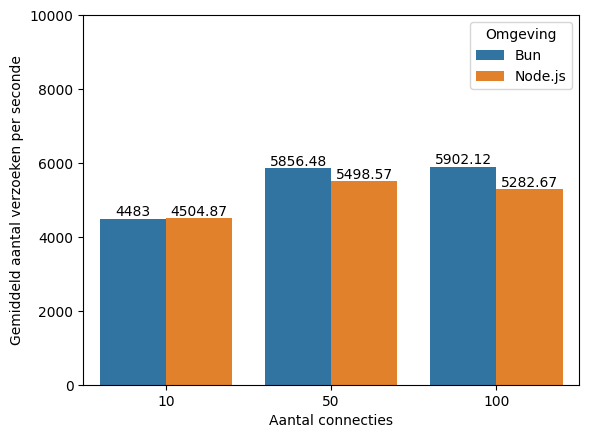
\includegraphics{graphics/PostMySqlVerzoeken.png}
      \caption{\label{fig:postaantalverzoekenmysql}Visuele voorstelling gemiddeld aantal verzoeken per seconde bij het maken van een recensie.}
    \end{figure}
    \begin{figure}[H]
      \centering
      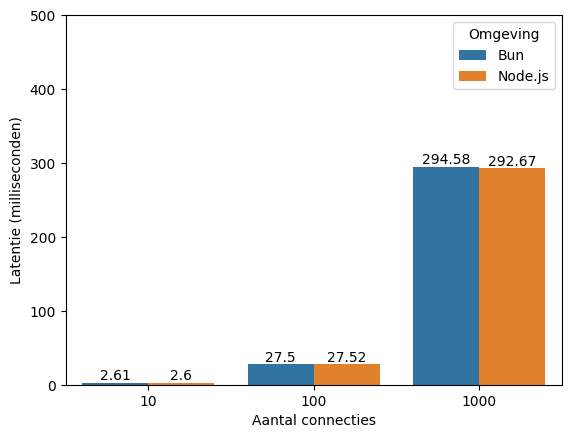
\includegraphics{graphics/PostMySqlLatentie.png}
      \caption{\label{fig:postaantallatentienmysql}Visuele voorstelling gemiddelde latentie bij het maken van een recensie.}
    \end{figure}
    \begin{figure}[H]
      \centering
      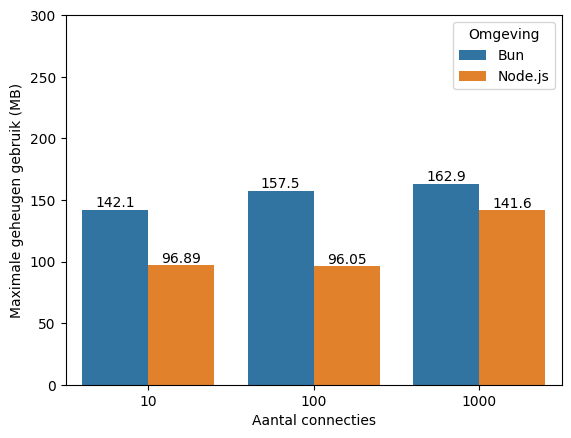
\includegraphics{graphics/PostMySqlRAM.png}
      \caption{\label{fig:postgeheugennmysql}Visuele voorstelling maximale geheugen gebruik bij het maken van een recensie.}
    \end{figure}
    \begin{figure}[H]
      \centering
      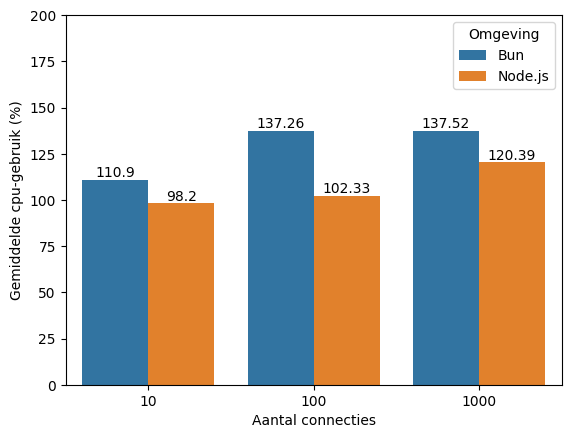
\includegraphics{graphics/PostMySqlCpu.png}
      \caption{\label{fig:postcpymysql}Visuele voorstelling gemiddeld CPU-gebruik bij het maken van een recensie.}
    \end{figure}

\subsection{Discussie}
Aan de hand van de Quick Sort algoritme resultaten kan het standpunt dat Bun computationeel sneller is ondersteund worden.
Zo was de gemiddelde uitvoeringstijd van Bun gemiddeld 2.21 keer sneller dan Node.js. Deze snellere uitvoeringstijd komt door de
het gebruik van de JavaScriptScore engine in Bun waarbij geoptimaliseerde machine code wordt geproduceerd in 
samenwerking met 3 JIT compilers en een Low-Level interpreter.
Deze snelheid is niet enkel zichtbaar bij het algoritme, maar ook bij de installatietijd van de packages.
Zo is Bun me teen gemiddelde installatietijd van 24,9 milliseconden 24,5 keer sneller is dan Node.js met een 
gemiddelde installatietijd van 610,1 milleseconden. Dit kan een groot verschil betekenen op vlak van efficiëntie in projecten met een groot aantal packages.
